\section{Building the Visualization}\label{sec:methodology}
{\color{Magenta}
The increasing role of technology in society means that the questions the project explores---namely, who gets to build our technologies and how effective the calls for diversity in tech have been---are relevant to the general public, not merely to those inside the tech world. Consequently, the project has three major goals:
\begin{enumerate}
  \item Connect prior research by presenting data on both education and employment in tech
  \item Facilitate comparison across datasets, even for those without sophisticated analytical skills
  \item Provide context to highlight the importance of interesting points within the data
\end{enumerate}
}

\subsection{Data Collection \& Cleaning}\label{sec:dev-data}
As discussed in \autoref{sec:design-data}, I used AP exam data from the College Board\footnote{AP Demographics available at \url{https://research.collegeboard.org/programs/ap/data}}, graduation data from the Taulbee Survey\footnote{Taulbee Survey available at \url{http://cra.org/resources/taulbee-survey/}}, and employment data from the U.S. Bureau of Labor Statistics\footnote{Labor Statistics available at \url{https://www.bls.gov/cps/tables.htm}}
 to construct the visualizations. \autoref{tbl:data-sources} summarizes the subset of each dataset used for this project.

\begin{table}
  \begin{tabular}{L{3.6cm}cL{4cm}l} \hline
    \textbf{Data Source} & \textbf{Years Included} & \textbf{Subset} & \textbf{Variables} \\ \hline
    \href{https://research.collegeboard.org/programs/ap/data}{College Board AP Demographics}
      & 2010--2016
      & AP Computer Science Exam
      & Gender, Exam Score \\
    \href{http://cra.org/resources/taulbee-survey/}{CRA's Taulbee Survey}
      & 2010--2015
      & Graduate \& Undergraduate degrees awarded
      & Gender, Program \\
    \href{https://www.bls.gov/cps/tables.htm}{United States Bureau of Labor Statistics Detailed Employment (Table 11)}
      & 2011--2015
      & Computing Occupations
      & Gender, Occupation \\ \hline
  \end{tabular}
  \caption{Summary of Data Sources Used}\label{tbl:data-sources}
\end{table}

Where feasible, I collected all data going back to 2010; the Bureau of Labor Statistics changed their reporting categories in 2011, so for consistency I excluded their 2010 data. Only the College Board had released 2016 data at the time of collection. Because not all groups contain the same years' data, visualizations including multiple groups use percentage breakdowns by gender, rather than absolute numerical comparisons.

All three data sources are available either as spreadsheets or in PDF tables. The College Board spreadsheets include demographic information for all AP tests, broken out by gender and by exam score, so I extracted the data for the Computer Science exam and discarded the others. The Bureau of Labor Statistics similarly includes all occupations in their spreadsheet, so I extracted the data for all of the ``Computer and Mathematical Occupations'' as seen in the literature. The Taulbee Survey publishes its data as part of an annual PDF report; because the data is already aggregated (and consequently fairly small), I manually copied the data from their PDFs into a CSV file.

Both the College Board and the Taulbee Survey give the aggregated counts of male and female students for each relevant category, so the only further processing required was to format each row consistently. The Bureau of Labor Statistics, on the other hand, provides a total count of employees for each category, rounded to the nearest thousand, along with the percentage of women employed in each category. They do not provide diversity statistics for categories with fewer than 50,000 total employees, so I excluded these categories from the visualization. For the categories included, I used the percentages of female employees to calculate an approximate female employee count, to better correspond with the data for educational stages.

\subsection{Early Design Sketches}\label{sec:dev-sketches}
\begin{figure}
  \centering
  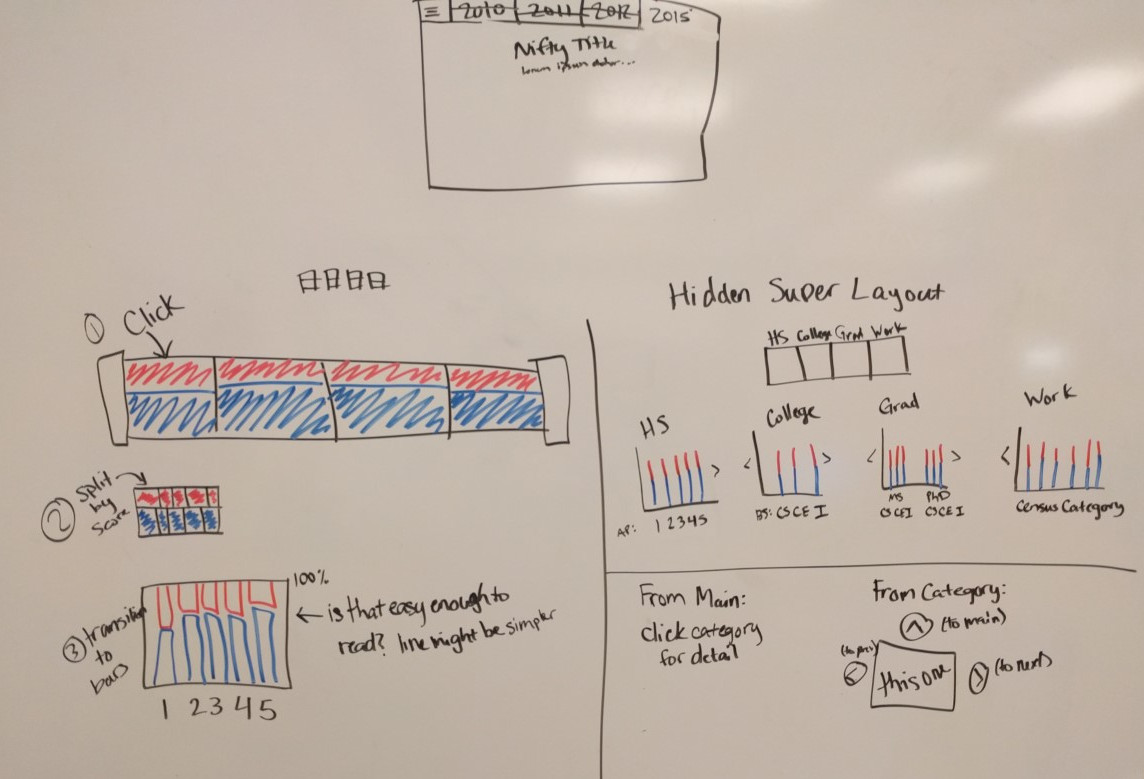
\includegraphics[width=0.8\textwidth]{whiteboard-1-layout}

  \vspace{0.1in}

  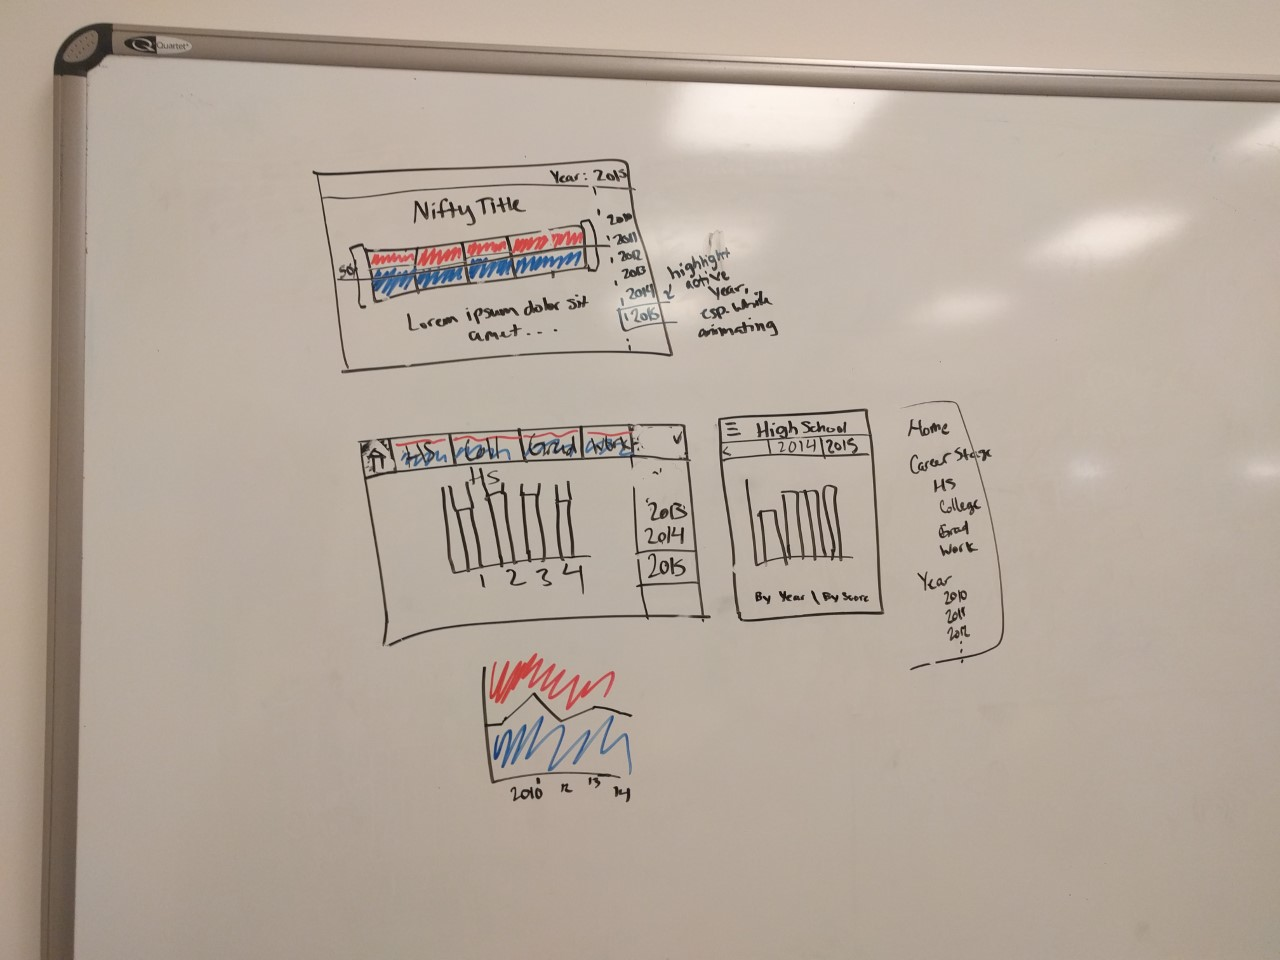
\includegraphics[width=0.8\textwidth]{whiteboard-2-navigation}
  \caption{Early Design Sketches: page layout (top) and alternate navigation (bottom)}\label{fig:whiteboard}
\end{figure}

I used low-fidelity whiteboard sketches to design and test early versions of the webpage before creating a code version. In the early designs, shown in \autoref{fig:whiteboard}, I focused on the visual relationship between the overview and the detailed views of each pipeline stage, on page navigation, and on graph types to display data. The top sketch shows disassembled overview of the page layout. The page frame at the top of the sketch uses a top navigation based on the stages of the tech education pipeline, so users interested in a particular stage can jump directly to it. To the left, it uses a pipe segment to visually represent the pipeline, which is divided into sections and color-coded according to the gender ratio of that section. The numbered sections below the pipe model a proposed animation from the overview into a bar graph for one of the detailed views. The right panel shows the spatial relationship between views, with vertical movement from the overview to each detailed view and horizontal movement between stages of the pipeline. This was intended to use the chronological nature of the pipeline to suggest a narrative on its own, connecting one stage of the pipeline to the next in the same way an individual would follow them throughout her career.

However, truly following the flow of a single career would require longitudinal data, which the combination of aggregated datasets cannot provide. Instead, the data supports viewing trends over time, so the bottom sketch explores ways to include time series information in the page navigation. The first panel introduces a drop-down menu to filter the entire display by year, with an option to animate through all available years. The next displays show alternatives for desktop and mobile views: on a large display, the top menu gets a series of colored backgrounds to mimic the color-coding of the overview pipe, with the same year filter as a dropdown. On smaller displays, the menu collapses into a hamburger pullout, and the year filter is present both within that menu and directly under the header, where it can be swiped sideways as needed. The bottom frame shows a color-coded area chart tracking the gender ratio over time.

The smudges in \autoref{fig:whiteboard} are evidence of my first round of testing, intended to determine whether the time-based navigation would make sense to viewers. Since this was a very preliminary test, I did not use rigorous standards for selecting participants or testing the layout: I asked nearby classmates who had no familiarity with my design goals if they would exchange feedback for a cookie. Two volunteered, so I brought them one at a time to the whiteboard, gave them a one-sentence introduction to the purpose of the site, and asked how they would interact with it. As they explained (or ``clicked'' on the whiteboard), I drew in details or menus, as needed.

Only one of the two found the drop-down without prompting, and she said she was unlikely to use a filter placed that far away from the graphs it applied to. The other participant simply wanted to scroll for more information.

\subsection{Refined Design Wireframes}\label{sec:dev-wireframes}
\begin{figure}
  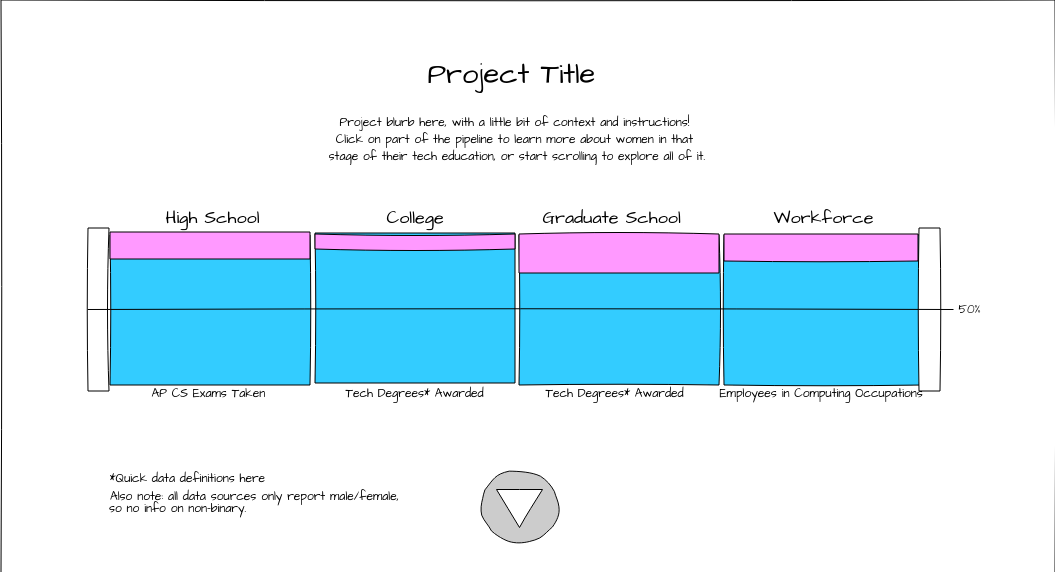
\includegraphics[width=\textwidth]{wireframe-1-overview}

  \vspace{2cm}

  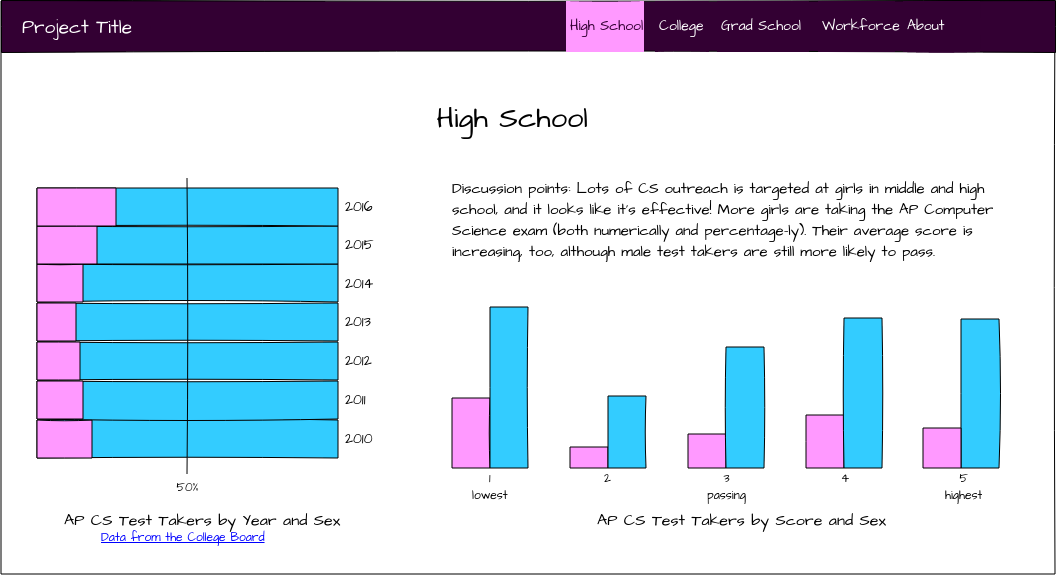
\includegraphics[width=\textwidth]{wireframe-2-hs-detail}
  \caption{Wireframes: overview (top) and high school detail (bottom)}\label{fig:wireframes}
\end{figure}

Since neither test participant found the time-based navigation useful, I removed it and simplified the page navigation for the next iteration of the design. Instead of a menu, viewers see a downward arrow indicating the page is scrollable; in this design, scrolling takes users from the overview to the detailed views, as well as from one detailed view to the next.

I also added narrative descriptions to each detailed view, to discuss issues unique to that stage in the pipeline and to highlight data of interest within that stage. I separated time series data and data by group (AP score, academic program, or specialized occupation) into two separate graphs, placed side-by-side, to show both the granular group data and the trends over time without relying on another menu. \autoref{fig:wireframes} shows the wireframes produced at the end of this refinement, made with the Pencil Prototyping tool\footnote{\url{http://pencil.evolus.vn/Next.html}}.

I performed another casual test at this point in the process, recruiting two new testers who roughly fit the personas presented in \autoref{sec:design-users}: a classmate interested in web development to represent Laurie's opinion, and an undergraduate communications major to represent Gabriella's. In addition to verifying that the simpler navigation was easier to understand, I used this test to compare ways of presenting the narrative elements. After explaining how they would interact with a page containing only the graphs and headings, they saw three different versions of the page: the same graphs-only layout, one with introductory text for each section, and one with annotations added to interesting points on the graph. The introductory texts were written on sticky notes and the annotations were on Post-It flags, so the two test layouts were of similar quality. Both testers preferred the version with introductory text pictured in the final wireframes, claiming the original version needed more explanation but that the annotations distracted from the graphs.


\subsection{Website Development}\label{sec:development}
\begin{figure}
  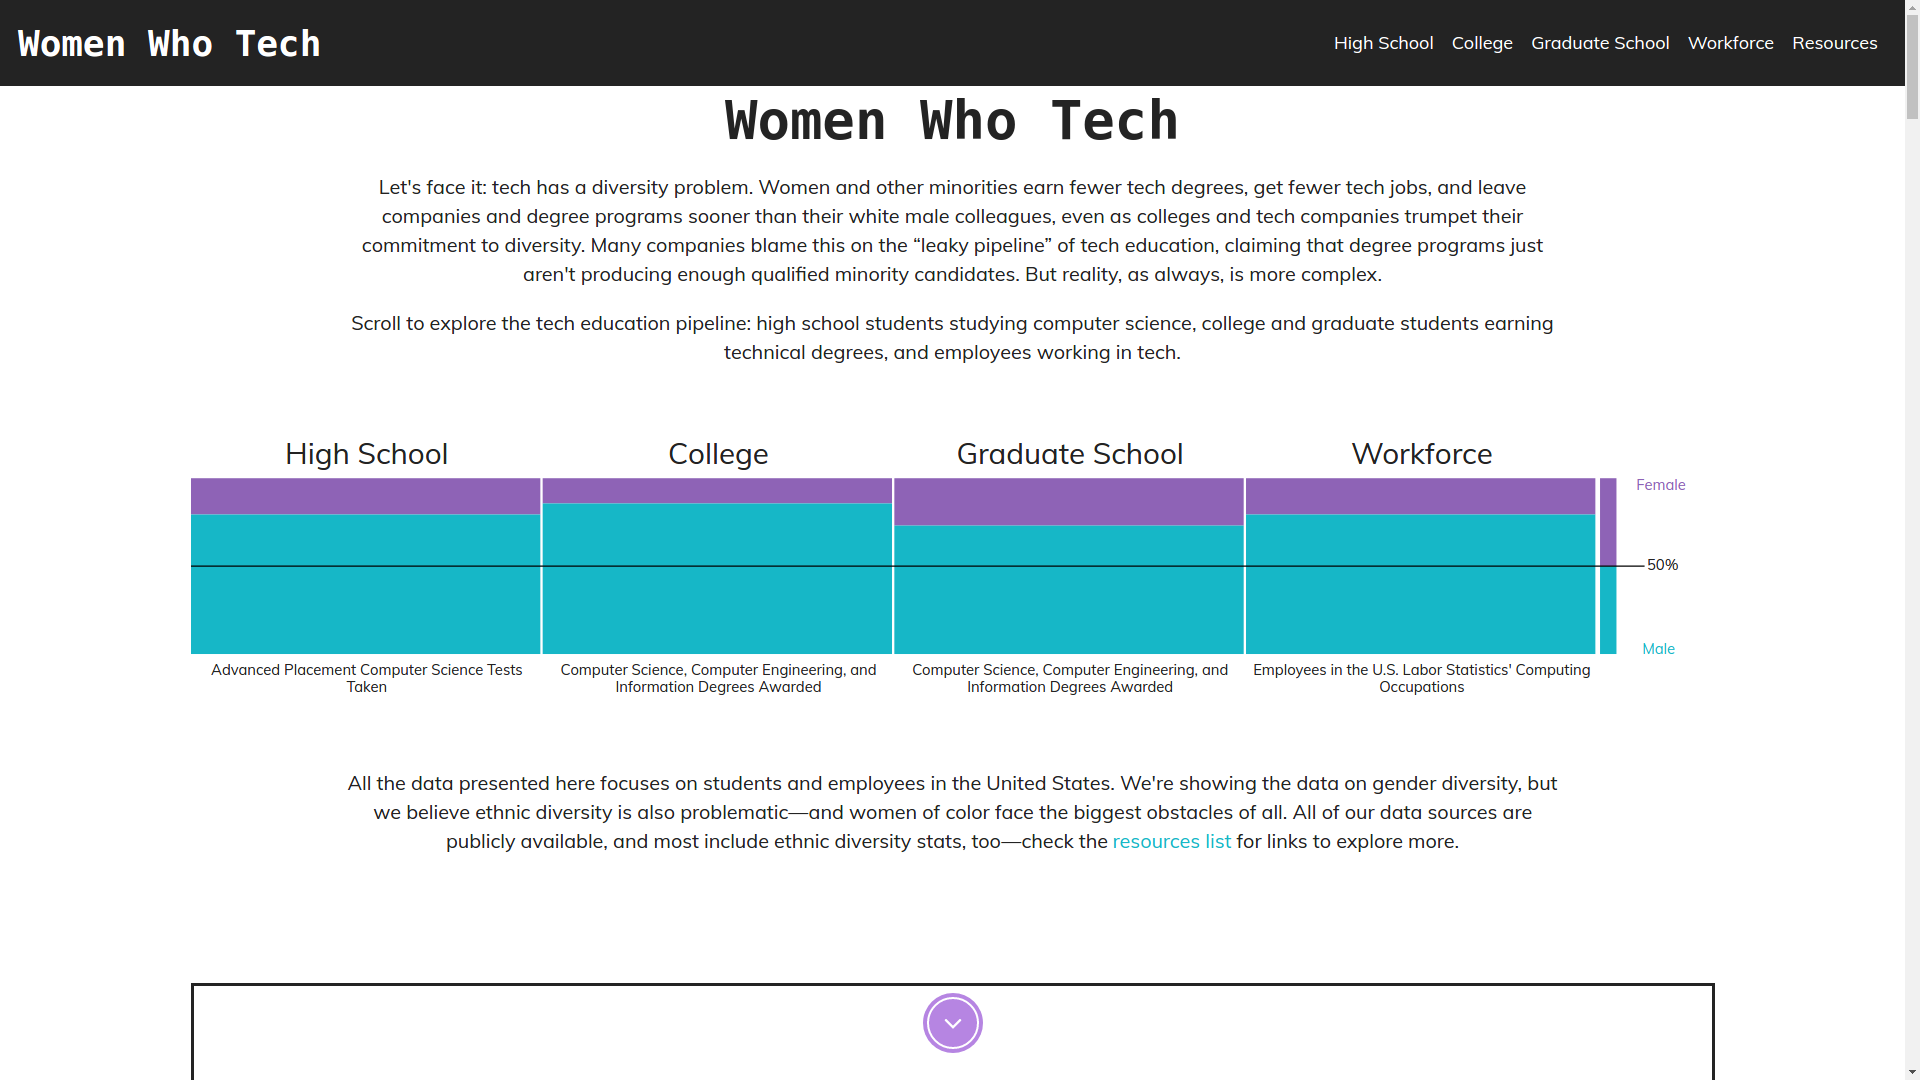
\includegraphics[width=0.95\textwidth]{screen-1-overview}


  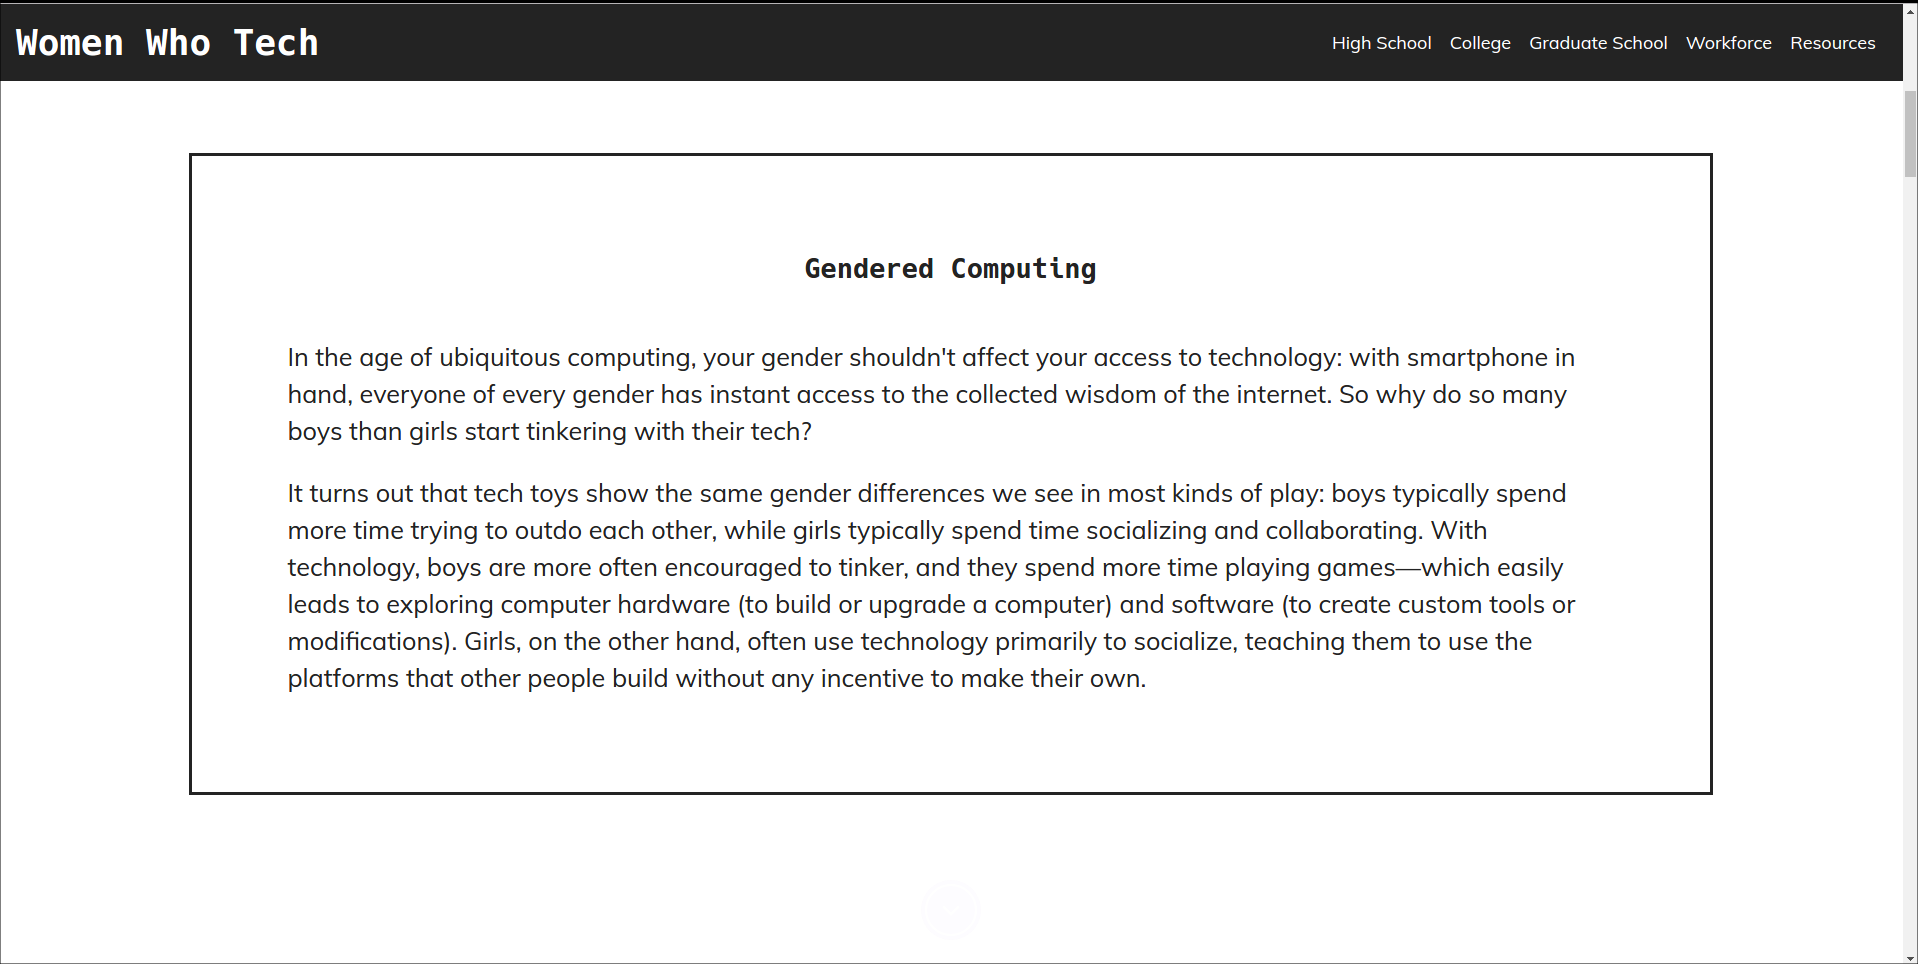
\includegraphics[width=0.95\textwidth]{screen-2-interlude}


  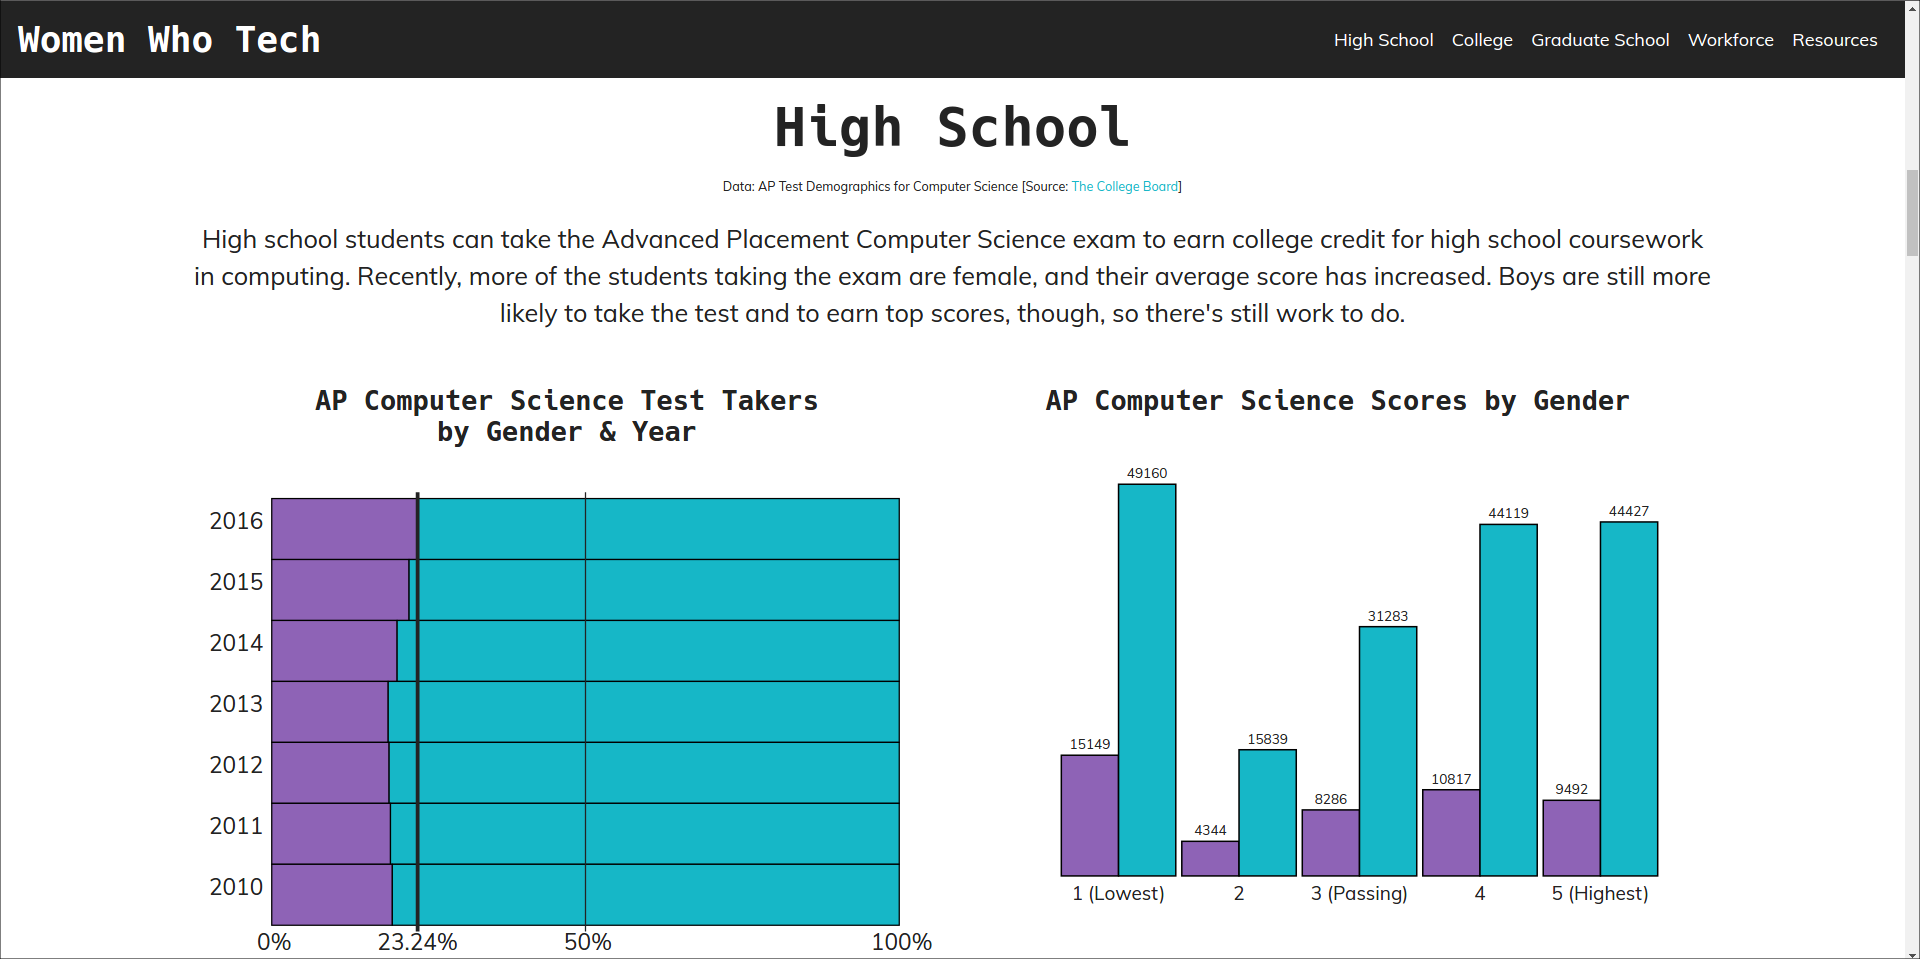
\includegraphics[width=0.95\textwidth]{screen-3-hs-detail}
  \caption{Screenshots: overview (top), narrative frame (middle), and high school detail (bottom)}\label{fig:screenshots}
\end{figure}

The actual webpage, shown in \autoref{fig:screenshots}, was constructed using HTML5/CSS3 for the page layout and the D3.js JavaScript library\footnote{\url{https://d3js.org/}} for the visualizations. The page display conforms to responsive web design principles, although the interactive aspects of the visualizations do not.

\textcolor{magenta}{EXPAND}
